\documentclass[11pt,a4paper]{article}

\usepackage[margin=1in]{geometry}
\usepackage{amsmath,amssymb,bm}
\usepackage{booktabs}
\usepackage{graphicx}
\usepackage{setspace}
\usepackage[numbers,sort&compress]{natbib}
\usepackage[hidelinks]{hyperref}
\usepackage{xcolor}

\onehalfspacing
\setlength{\emergencystretch}{1em}
\graphicspath{{figures/}}

\title{Low-Resource Nepali Sign Language Alphabet Recognition on NSL23:\\
An Exploratory Cross-Signer Study of RGB and Hand-Landmark Models}

\author{Shaswat Chapagain\\
University of California, Berkeley\\
\texttt{shaswat\_chapagain@berkeley.edu}}

\date{}

\begin{document}
\maketitle

\begin{abstract}
Public Nepali Sign Language (NSL) video is scarce, and published results use collections with different vocabularies and evaluation splits. We study isolated alphabet recognition on NSL23 using 375 original, individually labelled clips from seven signers. Aggregate recordings without gesture timestamps and cropped copies are excluded. S1 and S2, the only signers with a complete isolated alphabet, are held out in turn, with 277 training and 98 evaluation clips per fold. Five RGB and hand-landmark models share a 30-epoch, three-seed schedule. On 196 pooled cross-signer development clips, RGB accuracy ranges from $5.8\% \pm 0.8\%$ to $7.0\% \pm 2.1\%$, against $2.0\%$ uniform-guessing accuracy for 49 classes. A landmark BiLSTM using wrist-relative xyz reaches $24.8\% \pm 4.0\%$, with $66.0\% \pm 4.0\%$ on vowels and $10.0\% \pm 3.9\%$ on consonants. Adding 20 inter-joint angles and prototypical training~\cite{snell2017prototypical,chamachot2026geometry} gives $59.4\% \pm 3.3\%$ accuracy and $57.4\% \pm 3.6\%$ macro-F1, including $61.8\% \pm 5.7\%$ consonant accuracy. These are exploratory estimates: S1/S2 results informed the follow-on representation choices. The reported standard deviations describe variation across three training seeds, not uncertainty across the signer population. With one labelled support clip per class from the held-out signer's other lighting, cross-entropy BiLSTMs reach $76.2\%$--$78.2\%$ in a separate 49-way enrollment protocol. Recorded-video throughput tests of the CPU streaming loop reach $33$--$42$ frames per second on an Apple~M4; they do not measure live-camera recognition accuracy.
\end{abstract}

\noindent\textbf{Keywords:} Nepali Sign Language; NSL23; cross-signer development evaluation; hand landmarks; MediaPipe; prototypical networks; joint angles; webcam; low-resource sign recognition

\section{Introduction}

When the same person appears in training and test, a classifier may use clothing, background, or other signer-specific cues. Evaluating on a signer excluded from training tests transfer across people, although recording conditions may also change. Isolated-sign benchmarks such as MS-ASL, WLASL, and AUTSL use signer-independent partitions~\cite{vaezi2019msasl,li2020wlasl,sincan2020autsl}. NSL23 is much smaller than these collections.

NSL23 is a public alphabet collection released under CC~BY~4.0. It contains 36 consonants and 13 vowels~\cite{sunuwar2024nsl23,sunuwar2023zenodo}. The files are easy to overcount. The dataset paper reports 1,205 gesture instances in 630 videos. Some files are one labelled letter. Others are long aggregate takes. Others are cropped copies of an original. If every file, or every reported instance, is treated as an independent clip, the sample inflates and the same performance can leak across a split.

The original goal was a laptop-camera alphabet recognizer. The initial CNN--Transformer used letterboxed RGB, a compact MobileNetV2 encoder~\cite{sandler2018mobilenetv2}, and a temporal architecture used in sign-sequence modelling~\cite{camgoz2020sign,vaswani2017attention}. Under the fixed signer-held-out protocol, the RGB models scored only a few points above chance, while the temporal heads reached training accuracy 1.00. This gap motivated a comparison with hand-landmark features.

MediaPipe Hands returns 21 three-dimensional keypoints~\cite{zhang2020mediapipe}. The vector is small enough to classify on CPU, and it discards most of the clothing and background that a frozen ImageNet encoder still sees. NSL letter work has already used landmarks on other image sets~\cite{shrestha2024mediapipe}. Those papers did not score these original isolated clips with S1 and S2 held out.

The study keeps the 375 audited clips and the two held-out folds fixed. It compares frozen RGB encoders with landmark classifiers, then examines joint angles, prototypical training, 1-shot enrollment, and streaming throughput on the same files. Only two signers provide complete 49-class evaluation sets, and their results informed the follow-on choices. The percentages therefore describe an exploratory development sample. Heuju and Rijal's word-level Transformer~\cite{heuju2022word} and Shrestha et al.'s still-image letter CNN~\cite{shrestha2024mediapipe} used different collections and splits, so their scores are not directly ranked against these results. The geometric representation is inspired by Chamachot and Lertniphonphan~\cite{chamachot2026geometry}, rather than an exact replication of their static-alphabet system.

\section{Related work}

\subsection{Sign recognition and signer splits}

Video sign-recognition systems commonly combine spatial features with temporal models~\cite{rastgoo2021survey}. Sign Language Transformers jointly model continuous recognition and translation~\cite{camgoz2020sign}. Isolated benchmarks such as MS-ASL, WLASL, and AUTSL classify one sign and provide signer-independent partitions~\cite{vaezi2019msasl,li2020wlasl,sincan2020autsl}. Their scores cover different languages and vocabularies. This study adopts signer separation while retaining the NSL23 alphabet and source files.

\subsection{Nepali Sign Language systems}

Most published NSL systems use private collections. Heuju and Rijal trained Transformer and CNN--RNN models on word videos with a 70/30 split and reported $55.9\%$ on 71 words versus $89\%$ on a nine-word subset~\cite{heuju2022word}. Shrestha et al.\ used MediaPipe landmarks and a CNN on their own letter images~\cite{shrestha2024mediapipe}. Attention and landmarks have both been tried for NSL. Neither paper scores the original isolated NSL23 clips. Model comparisons in this study stay on the same held-out files.

The NSL23 dataset paper identifies Sikkim Manipal Institute of Technology in Sikkim, India, as the data source location~\cite{sunuwar2024nsl23}. This study reuses that collection. Evaluating use in Nepal would require additional locally collected data.

\subsection{Lightweight RGB encoders and pose}

MobileNetV2 is a compact ImageNet classifier~\cite{sandler2018mobilenetv2}. Pretrained visual features sometimes transfer; how well they transfer depends on the domain gap~\cite{kornblith2019better}. Isolated NSL letters are hand shapes, often nearly static, shot at mixed resolutions. An ImageNet encoder is frozen as a controlled baseline, even though ImageNet features are a weak description of these hands. Pose pipelines replace the image with keypoints. MediaPipe Hands is built for on-device tracking~\cite{zhang2020mediapipe}. It misses under occlusion, blur, and poor light. Those misses are left in the features rather than swapping detectors after seeing errors.

\subsection{Geometric hand features and prototypical classifiers}

Wrist-relative coordinates retain hand orientation. Angles between nonzero vectors are invariant to a common rigid rotation, translation, and uniform scale of the supplied points. This mathematical property does not guarantee invariance to camera viewpoint or detector error in image-derived landmarks; the concatenated xyz+angle representation also retains orientation through its xyz component. Chamachot and Lertniphonphan use a 20-angle descriptor with a prototypical network on static fingerspelling images~\cite{chamachot2026geometry}. Prototypical networks compare a query with class-mean embeddings~\cite{snell2017prototypical}. Here, a BiLSTM encodes 16-frame NSL23 sequences, and classification uses unsquared Euclidean distance.

\section{Dataset and evaluation protocol}

\subsection{Release audit}

NSL23 version~2 was downloaded from the official Zenodo record~\cite{sunuwar2023zenodo}. Byte sizes and MD5 digests of the four archives and the dataset-detail document match the record. A file-level manifest retains archive, path, signer token, filename, canonical class, recording descriptors, and exclusion reason.

The audit counts 630 decodable videos: 607 individually labelled files and 23 aggregate recordings. The distribution also contains 234 cropped or preprocessed files. The primary sample is the complement of both exclusions: 375 original, individually labelled clips from S1, S2, S7, S8, S10, S11, and S12 (Figure~\ref{fig:flow}). All 49 alphabet classes appear in that set.

\begin{table}[t]
\centering
\caption{Audited NSL23 counts used in this study. ``Instances'' in the source article are not separately labelled clips.}
\label{tab:audit}
\small
\begin{tabular}{lc}
\toprule
Quantity & Count \\
\midrule
Decodable videos in the release & 630 \\
Individually labelled files & 607 \\
Aggregate recordings (no timestamps) & 23 \\
Cropped or preprocessed files & 234 \\
Primary original isolated clips & 375 \\
Primary signers & 7 \\
Alphabet classes & 49 \\
Training clips per fold & 277 \\
Test clips per fold (S1 or S2) & 98 \\
Seeds $\times$ models $\times$ folds & $3 \times 5 \times 2 = 30$ runs \\
\bottomrule
\end{tabular}
\end{table}

\begin{figure}[t]
\centering
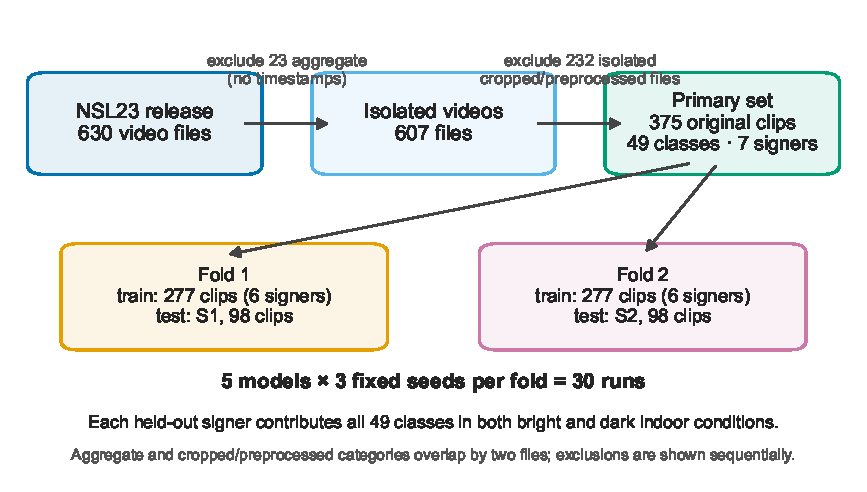
\includegraphics[width=0.98\linewidth]{figure_1_study_flow.pdf}
\caption{From the NSL23 release to the 30-run matrix. Aggregate files and cropped derivatives are removed before the two signer-held-out folds.}
\label{fig:flow}
\end{figure}

Aggregate recordings were opened and watched. Filenames were ignored as labels. The release has no per-gesture timestamps. Equal-duration bins in published alphabet order drift; at least one sequence appears incomplete or shifted. An equal-duration cut can therefore assign the wrong class while still showing a plausible hand. Those bins are never used as labels.

Cropped copies are excluded so that a derived rendering of the same take cannot sit in the opposite fold, and so that every prediction points at one original file.

\subsection{Class list and folds}

The ontology is 36 consonants followed by 13 vowels. Filename aliases are resolved with signer-aware rules because the release uses more than one transliteration. The label set stays at those 49 letters. Every test clip has a class that also appears in training, and each fold contains all 49 labels on both sides of the split.

Only S1 and S2 have original isolated clips for the full alphabet. Fold~1 trains on S2, S7, S8, S10, S11, and S12 and tests on S1. Fold~2 swaps S1 into training and tests on S2. Each test signer contributes one bright and one dark original clip per class. There is no validation set and no early stopping. The epoch-30 checkpoint is evaluated once per run.

The folds are uneven by sign type. S7, S8, S10, S11, and S12 contribute prepared consonants only. Isolated vowels exist only for S1 and S2, so each fold learns every vowel from the other complete-alphabet signer. A correct vowel prediction therefore crosses a one-to-one signer boundary. Consonant training has more signers. The test person remains absent from training, but the broad unprepared indoor condition is represented by the other complete-alphabet signer.

\subsection{Frame sampling}

Sixteen frames are taken at the centres of equal temporal bins of each clip, resized with aspect ratio preserved, and letterboxed to $224 \times 224$. ImageNet channel mean and standard deviation are applied at load time. Training uses brightness and contrast perturbations drawn once per clip and applied to all 16 frames. Horizontal flipping is disabled. The single-frame CNN uses the middle element of the same 16-frame sample.

\section{Methods}

Figure~\ref{fig:arch} shows the two pipelines. RGB models share a frozen encoder. Landmark models share MediaPipe Hands and a wrist-relative 64-dimensional frame vector.

\begin{figure}[t]
\centering
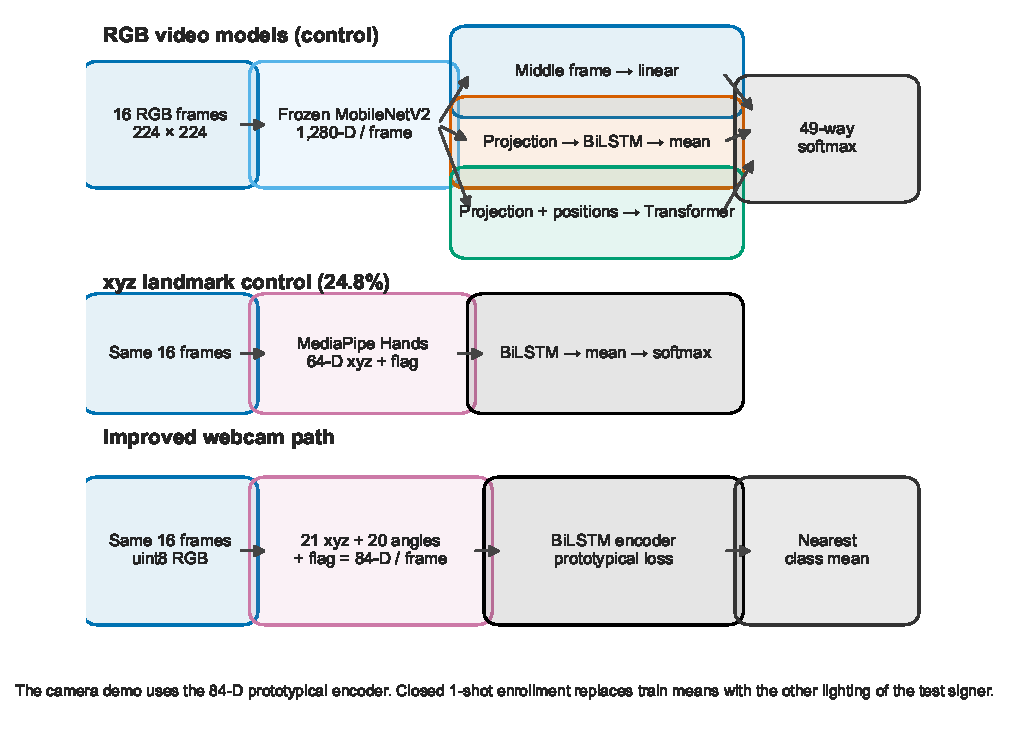
\includegraphics[width=0.98\linewidth]{figure_2_architectures.pdf}
\caption{RGB controls (top), xyz landmark softmax (middle), and the improved webcam path (bottom): 84-D xyz+angle frames and nearest class prototype.}
\label{fig:arch}
\end{figure}

\subsection{Frozen RGB models}

Let a clip be $\mathbf{X} \in \mathbb{R}^{T \times 3 \times 224 \times 224}$ with $T=16$. A frozen MobileNetV2 encoder $f_{\theta}$ with ImageNet-1K~V2 weights maps each frame to $\mathbf{z}_t \in \mathbb{R}^{1280}$~\cite{sandler2018mobilenetv2}. Encoder weights and batch-normalization running statistics are not updated.

The single-frame CNN classifies the middle frame:
\begin{equation}
\mathbf{h} = f_{\theta}(\mathbf{X}_{\lfloor T/2 \rfloor+1}), \qquad
\hat{\mathbf{y}} = \mathrm{softmax}(W \,\mathrm{Dropout}(\mathbf{h}) + b).
\end{equation}
With one-based indexing, this is the ninth of the 16 sampled frames. It has $62{,}769$ trainable parameters.

The CNN--BiLSTM projects $\mathbf{z}_t$ to $\mathbf{u}_t \in \mathbb{R}^{256}$, applies a one-layer bidirectional LSTM with 128 units per direction~\cite{hochreiter1997lstm}, layer-normalizes the outputs, and mean-pools time:
\begin{equation}
\mathbf{u}_t = W_p \mathbf{z}_t + b_p, \qquad
[\overrightarrow{\mathbf{h}}_t; \overleftarrow{\mathbf{h}}_t] = \mathrm{LSTM}(\mathbf{u}_{1:T}), \qquad
\bar{\mathbf{h}} = \frac{1}{T}\sum_{t=1}^{T} \mathrm{LN}([\overrightarrow{\mathbf{h}}_t; \overleftarrow{\mathbf{h}}_t]).
\end{equation}
It has $736{,}305$ trainable parameters.

The CNN--Transformer uses the same projection, adds a learned positional table $\mathbf{P} \in \mathbb{R}^{T \times 256}$, and applies two encoder layers with four heads and feed-forward width 512~\cite{vaswani2017attention}:
\begin{equation}
\mathbf{H} = \mathrm{Transformer}(\mathbf{U} + \mathbf{P}), \qquad
\bar{\mathbf{h}} = \frac{1}{T}\sum_{t=1}^{T} \mathrm{LN}(\mathbf{h}_t).
\end{equation}
Each head computes $\mathrm{softmax}(QK^{\top}/\sqrt{d_h})V$ with $d_h = 64$. Encoder dropout is $0$ (deterministic scaled-dot-product attention on the training host). Head dropout is $0.2$. There is no class token and no causal mask. The model has $1{,}399{,}345$ trainable parameters.

\subsection{Hand-landmark models}

MediaPipe Hands~\cite{zhang2020mediapipe} is run on the same 16 cached RGB frames (\texttt{static\_image\_mode=True}, complexity~1, at most two hands, detection confidence $0.35$). If several hands are returned, the hand with the highest handedness-classification confidence is kept. This score measures confidence in the left/right classification, rather than landmark accuracy.

Let $\mathbf{l}_i \in \mathbb{R}^{3}$ be the image-normalized coordinates of landmark $i \in \{0,\ldots,20\}$, with $i=0$ the wrist and $i=9$ the middle-finger metacarpophalangeal joint. Wrist-relative, scale-normalized features are
\begin{equation}
\mathbf{p}_i = \mathbf{l}_i - \mathbf{l}_0, \qquad
s = \lVert \mathbf{p}_{9}^{(x,y)} \rVert_2, \qquad
\tilde{\mathbf{p}}_i = \frac{\mathbf{p}_i}{s_*}, \qquad
s_* = \begin{cases}s,&s\geq\varepsilon,\\1,&s<\varepsilon,\end{cases}
\end{equation}
with $\varepsilon = 10^{-6}$. The frame vector concatenates the 63 coordinates and a detection flag $d_t \in \{0,1\}$:
\begin{equation}
\mathbf{x}_t = \bigl[\tilde{\mathbf{p}}_0;\ldots;\tilde{\mathbf{p}}_{20}; d_t\bigr] \in \mathbb{R}^{64}.
\end{equation}
A miss yields the zero vector, including $d_t=0$. No class-conditional imputation is used.

On the 375 primary clips ($6{,}000$ frames), Hands detected a hand in $5{,}868$ frames ($97.8\%$). No clip had zero detections. Primary cross-entropy training adds isotropic Gaussian noise with standard deviation $0.02$ to the 63 spatial coordinates, including initially zero coordinates on missed frames; the flag is not noised. Evaluation uses the unperturbed cache.

The landmark MLP flattens the clip to $\mathbb{R}^{1024}$ and uses hidden widths $256$ and $128$ with ReLU and dropout $0.3$ ($301{,}617$ parameters). The landmark BiLSTM is a one-layer bidirectional LSTM with 64 units per direction, layer normalization, temporal mean pooling, and dropout $0.3$ ($73{,}137$ parameters):
\begin{equation}
[\overrightarrow{\mathbf{h}}_t; \overleftarrow{\mathbf{h}}_t] = \mathrm{LSTM}(\mathbf{x}_{1:T}), \qquad
\bar{\mathbf{h}} = \frac{1}{T}\sum_{t=1}^{T} \mathrm{LN}([\overrightarrow{\mathbf{h}}_t; \overleftarrow{\mathbf{h}}_t]).
\end{equation}

\subsection{Joint angles and prototypical training}

The follow-on matrix keeps the same 16-frame MediaPipe cache. Inspired by the geometric descriptor of Chamachot and Lertniphonphan~\cite{chamachot2026geometry}, our implementation computes 15 intra-finger flexion angles and five span angles at the wrist. The five landmark chains are $(0,1,2,3,4)$, $(0,5,6,7,8)$, $(0,9,10,11,12)$, $(0,13,14,15,16)$, and $(0,17,18,19,20)$; each contributes its three consecutive triplets. The wrist triplets (parent, pivot, child) are $(1,0,5)$, $(5,0,9)$, $(9,0,13)$, $(13,0,17)$, and $(1,0,17)$. For unit vectors $\mathbf{u}$ and $\mathbf{v}$ from a pivot joint,
\begin{equation}
\phi(\mathbf{u},\mathbf{v}) = \arccos\bigl(\mathrm{clip}(\mathbf{u}^{\top}\mathbf{v}, -1, 1)\bigr).
\end{equation}
A vector with norm below $10^{-8}$ yields angle zero; a missed hand ($d_t=0$) yields a zero angle vector. Unlike the cited static-image system, this implementation uses wrist-to-middle-finger scale normalization, a detection flag, temporal BiLSTM encoding, and unsquared Euclidean distance. Concatenating the 63 coordinates, the 20 angles, and the detection flag gives
\begin{equation}
\mathbf{x}_t^{\mathrm{raw+ang}} = \bigl[\tilde{\mathbf{p}}_0;\ldots;\tilde{\mathbf{p}}_{20}; \boldsymbol{\phi}_t; d_t\bigr] \in \mathbb{R}^{84}.
\end{equation}
The BiLSTM input width grows from 64 to 84 ($83{,}377$ parameters). The cross-entropy loader adds Gaussian noise with standard deviation $0.02$ to all non-flag features after angle computation, so both coordinates and angles receive jitter in this follow-on representation.

Prototypical training uses the same BiLSTM as an encoder $g_{\psi}$ that maps a clip to $\bar{\mathbf{h}} \in \mathbb{R}^{128}$. Each epoch runs 40 episodes. An episode draws, for every class, five support clips and two query clips from the training fold, with replacement when a class has fewer than seven training clips. Class prototypes are support means. The loss is softmax over Euclidean distances~\cite{snell2017prototypical}:
\begin{equation}
\mathbf{c}_c = \frac{1}{|S_c|}\sum_{(\mathbf{X},y)\in S_c} g_{\psi}(\mathbf{X}), \qquad
p(y=c\mid\mathbf{X}) = \frac{\exp(-\lVert g_{\psi}(\mathbf{X})-\mathbf{c}_c\rVert_2)}{\sum_{c'}\exp(-\lVert g_{\psi}(\mathbf{X})-\mathbf{c}_{c'}\rVert_2)}.
\end{equation}
After 40 epochs, test clips are classified by nearest \emph{training}-set prototype. The held-out signer never contributes a prototype in this evaluation. An xyz-only prototypical ablation uses the same encoder and episodes with 64-D frames. Sampling with replacement can place the same training clip in both support and query sets within an episode, particularly for the two-clip vowel classes. The reported five support and two query draws therefore need not be distinct examples. Evaluation clips remain separate from training.

\subsection{Cropped-hand CNN and fusion}

Full-frame RGB leaves the hand as a small region in a $224\times 224$ letterbox. A follow-on control crops a square around the detected hand from the same 16 cached frames, resizes the crop to $224\times 224$, and trains the frozen MobileNetV2 middle-frame classifier on those crops ($62{,}769$ trainable parameters). Fusion averages softmax probabilities from a landmark model and the crop CNN with equal weight. Like the other follow-on comparisons, it is exploratory.

\subsection{Closed 1-shot enrollment}

Each test signer has two original clips per class (bright and dark), which is too few for 5-shot enrollment of that person. The 1-shot protocol runs two directions per signer: 49 dark clips support 49 bright queries, then 49 bright clips support 49 dark queries. Pooling the two directions gives 98 query predictions per signer. Every class prototype in each direction comes from that signer. An alternative replaces only the known true class prototype and keeps the other 48 training-class means. It uses the query label to construct its candidate set and is excluded from reported enrollment results.

\subsection{Loss and optimization}

The five models in the primary matrix use inverse-frequency class-weighted cross entropy without label smoothing. For class counts $n_c$ in a training fold,
\begin{equation}
w_c \propto \frac{1}{n_c}, \qquad
\frac{1}{C}\sum_{c=1}^{C} w_c = 1, \qquad
\mathcal{L} = -\sum_{c=1}^{C} w_c \, y_c \log \hat{y}_c,
\end{equation}
with $C=49$. This is the per-example weighted loss; PyTorch's batch mean divides the sum of example losses by the sum of their target-class weights. The weights offset the release's two isolated clips per vowel versus up to seven per consonant.

AdamW uses learning rate $3 \times 10^{-4}$ and weight decay $10^{-4}$~\cite{loshchilov2019adamw}, with cosine annealing over 30 epochs, batch size 8, and seeds $17$, $42$, and $73$. Deterministic algorithms are enabled. RGB models train on Apple~M4 MPS; landmark models train on CPU. This controls supported nondeterministic operations on the recorded host, but it does not promise bitwise identity across PyTorch releases, hardware, or devices. The schedule, including the absence of a validation split, was fixed before the RGB matrix and reused for landmarks. Prototypical runs use AdamW with the same initial learning rate, weight decay, and seeds for 40 epochs, but keep the learning rate constant and do not add feature jitter. Their episode loss is unweighted because every class contributes the same number of query draws. Loss, schedule, sampling, and augmentation therefore change together; this is not a loss-only ablation.

\subsection{Webcam loop}

The demo classifies a rolling window of live or replayed frames. It keeps the latest $T=16$ landmark vectors from a camera or video stream, concatenates the 20 joint angles, runs the prototypical BiLSTM, and assigns the nearest stored training-class mean. Class probabilities are a softmax over negated distances, optionally smoothed with an exponential moving average
\begin{equation}
\mathbf{s}_t = \alpha \mathbf{s}_{t-1} + (1-\alpha)\hat{\mathbf{y}}_t, \qquad \alpha = 0.4.
\end{equation}
Streaming speed is wall-clock frames processed per second, MediaPipe included. RGB clip throughput after offline decoding is reported separately.

\section{Experiments}

The primary matrix is five models, two folds, and three seeds (30 runs). On the same folds and seeds the follow-on matrix trains xyz+angle cross-entropy models, prototypical BiLSTMs (xyz and xyz+angle), and the cropped-hand CNN, then scores closed 1-shot enrollment. Reusing S1/S2 to motivate and compare these follow-on representations makes the complete matrix exploratory; ``held out'' means absent from a particular training run, not untouched by study-level model development. For the prototypical encoder we also record top-3, top-5, a 36-consonant restriction, five-class episodes using full training-class means, and same-signer 5-way 1-shot episodes. Checkpoints are never selected on these alternative evaluations. Each evaluation fold has 98 clips (49 classes $\times$ \{bright, dark\}). Seed-level scores pool the two held-out signers (196 unique clips). Architectures are summarized by the mean and sample standard deviation of the three seed scores. Top-1 accuracy and macro-F1 are the main descriptors~\cite{sokolova2009measures}. Equal class support makes pooled accuracy the same number as macro-recall.

Each run stores class-stratified clip bootstrap intervals (2{,}000 replicates). They describe prediction variability on these clips~\cite{efron1993bootstrap}. Two held-out signers are too few for those intervals to stand in for a population of signers.

Bright/dark and consonant/vowel splits were locked before the RGB matrix. Illumination was never randomized as an experimental factor. Architecture differences are seed-matched percentage points. Three seeds are too few for a hypothesis test.

RGB batch-one latency used Apple~M4 MPS with device synchronization: model-only forward pass versus original-video decode, preprocess, and inference. Landmark clip latency used CPU: model-only versus MediaPipe on 16 cached frames plus the classifier. The webcam loop was timed on original NSL23 \texttt{.MOV} files with the display off.

\subsection{Reproducibility boundary}

Before the first full primary run, 15 protocol, configuration, manifest, loader, model, training, and launcher files were recorded in a dated SHA-256 snapshot. A one-epoch software smoke test had already accessed the S1 evaluation fold before this snapshot; the chronology receipt records that its scores were not used for design or selection. The original snapshot did not capture its Git revision. A later audit found that every recorded byte and size matches Git commit \texttt{0eb1ff2} exactly, now named by the convenience tag \texttt{v1-protocol-freeze}. The dated hash snapshot remains the chronology record; the later tag is not a preregistration. A standalone verifier checks that historical Git tree, while a separate worktree mode reports subsequent edits as drift. Active manifests use repository-relative paths; historical run receipts retain the machine paths recorded when those runs occurred.

\section{Results}

\subsection{RGB controls}

Table~\ref{tab:primary} and Figure~\ref{fig:perf} summarize pooled scores. The single-frame CNN reaches $5.8\% \pm 0.8\%$ accuracy and $3.5\% \pm 0.2\%$ macro-F1. CNN--BiLSTM is $7.0\% \pm 2.1\%$ / $4.2\% \pm 2.1\%$. CNN--Transformer is $6.3\% \pm 0.8\%$ / $4.4\% \pm 1.3\%$. All three observed means exceed the $2.0\%$ uniform-guessing baseline, but each leaves more than nine in ten clips misclassified.

Seed-matched gaps among the RGB models are small (Transformer minus single-frame: $+0.5 \pm 1.0$ accuracy points). Both temporal RGB heads reach mean training accuracy $1.00$ by the last epoch (Figure~\ref{fig:train}), while evaluation accuracy stays near $6\%$. This indicates overfitting, although these measurements do not identify which visual cues the models use.

% Auto-generated from artifacts/results. Do not edit by hand.
\begin{table}[t]
\centering
\caption{Pooled unseen-signer performance (196 clips/seed; mean $\pm$ SD over three seeds). Chance accuracy for 49 classes is $2.0\%$.}
\label{tab:primary}
\small
\begin{tabular}{lcccc}
\toprule
Model & Acc. (\%) & Macro-P (\%) & Macro-R (\%) & Macro-F1 (\%) \\
\midrule
Single-frame CNN & 5.8 $\pm$ 0.8 & 3.6 $\pm$ 0.6 & 5.8 $\pm$ 0.8 & 3.5 $\pm$ 0.2 \\
CNN--BiLSTM & 7.0 $\pm$ 2.1 & 5.2 $\pm$ 5.0 & 7.0 $\pm$ 2.1 & 4.2 $\pm$ 2.1 \\
CNN--Transformer & 6.3 $\pm$ 0.8 & 5.7 $\pm$ 1.6 & 6.3 $\pm$ 0.8 & 4.4 $\pm$ 1.3 \\
Landmark MLP & 18.0 $\pm$ 2.1 & 10.3 $\pm$ 1.5 & 18.0 $\pm$ 2.1 & 11.1 $\pm$ 1.8 \\
Landmark BiLSTM & 24.8 $\pm$ 4.0 & 17.1 $\pm$ 5.6 & 24.8 $\pm$ 4.0 & 16.8 $\pm$ 3.8 \\
\bottomrule
\end{tabular}
\end{table}

\begin{table}[t]
\centering
\caption{Held-out signer accuracy and macro-F1 (98 clips/fold; mean $\pm$ SD over three seeds).}
\label{tab:folds}
\small
\begin{tabular}{lcccc}
\toprule
Model & S1 acc. (\%) & S1 F1 (\%) & S2 acc. (\%) & S2 F1 (\%) \\
\midrule
Single-frame CNN & 6.5 $\pm$ 0.6 & 2.8 $\pm$ 0.9 & 5.1 $\pm$ 1.0 & 2.9 $\pm$ 1.3 \\
CNN--BiLSTM & 8.2 $\pm$ 2.0 & 5.0 $\pm$ 3.2 & 5.8 $\pm$ 2.4 & 2.0 $\pm$ 1.1 \\
CNN--Transformer & 5.1 $\pm$ 1.0 & 3.7 $\pm$ 1.3 & 7.5 $\pm$ 1.2 & 3.0 $\pm$ 1.4 \\
Landmark MLP & 18.7 $\pm$ 3.1 & 11.6 $\pm$ 2.5 & 17.3 $\pm$ 1.0 & 10.1 $\pm$ 0.7 \\
Landmark BiLSTM & 25.9 $\pm$ 2.6 & 17.4 $\pm$ 2.0 & 23.8 $\pm$ 5.6 & 15.0 $\pm$ 4.8 \\
\bottomrule
\end{tabular}
\end{table}

\begin{table}[t]
\centering
\caption{Descriptive bright versus dark accuracy (98 pooled clips/condition/seed).}
\label{tab:lighting}
\small
\begin{tabular}{lcccc}
\toprule
Model & Bright acc. (\%) & Dark acc. (\%) & Bright F1 (\%) & Dark F1 (\%) \\
\midrule
Single-frame CNN & 5.8 $\pm$ 1.6 & 5.8 $\pm$ 0.6 & 3.2 $\pm$ 1.1 & 3.0 $\pm$ 0.7 \\
CNN--BiLSTM & 7.1 $\pm$ 1.0 & 6.8 $\pm$ 3.3 & 3.6 $\pm$ 1.6 & 4.0 $\pm$ 3.2 \\
CNN--Transformer & 7.1 $\pm$ 0.0 & 5.4 $\pm$ 1.6 & 4.5 $\pm$ 0.3 & 3.0 $\pm$ 1.5 \\
Landmark MLP & 21.4 $\pm$ 2.0 & 14.6 $\pm$ 2.1 & 12.7 $\pm$ 2.5 & 8.8 $\pm$ 1.2 \\
Landmark BiLSTM & 27.6 $\pm$ 3.5 & 22.1 $\pm$ 4.6 & 18.4 $\pm$ 3.1 & 14.3 $\pm$ 4.1 \\
\bottomrule
\end{tabular}
\end{table}

\begin{table}[t]
\centering
\caption{Consonant versus vowel accuracy on the pooled out-of-fold clips.}
\label{tab:signtype}
\small
\begin{tabular}{lcccc}
\toprule
Model & Cons. acc. (\%) & Vowel acc. (\%) & Cons. F1 (\%) & Vowel F1 (\%) \\
\midrule
Single-frame CNN & 4.2 $\pm$ 0.7 & 10.3 $\pm$ 2.2 & 2.8 $\pm$ 0.5 & 10.9 $\pm$ 2.6 \\
CNN--BiLSTM & 5.6 $\pm$ 1.8 & 10.9 $\pm$ 2.9 & 4.2 $\pm$ 1.8 & 8.8 $\pm$ 3.5 \\
CNN--Transformer & 4.9 $\pm$ 0.7 & 10.3 $\pm$ 2.9 & 4.0 $\pm$ 0.8 & 9.5 $\pm$ 2.6 \\
Landmark MLP & 7.2 $\pm$ 2.4 & 48.1 $\pm$ 1.9 & 5.6 $\pm$ 2.5 & 45.0 $\pm$ 2.8 \\
Landmark BiLSTM & 10.0 $\pm$ 3.9 & 66.0 $\pm$ 4.0 & 8.4 $\pm$ 4.0 & 64.2 $\pm$ 2.7 \\
\bottomrule
\end{tabular}
\end{table}

\begin{table}[t]
\centering
\caption{Batch-one clip latency. RGB end-to-end includes original-video decode on Apple M4 MPS. Landmark end-to-end is MediaPipe Hands on 16 cached frames plus the CPU classifier. Streaming FPS is reported separately.}
\label{tab:runtime}
\small
\begin{tabular}{lcccc}
\toprule
Model & Device & Model-only (ms) & End-to-end (ms) & Clips/s \\
\midrule
Single-frame CNN & MPS & 4.0 (4.2) & 939.0 (2097.8) & 1.06 \\
CNN--BiLSTM & MPS & 49.5 (50.2) & 962.9 (2126.2) & 1.04 \\
CNN--Transformer & MPS & 49.7 (50.1) & 970.9 (2162.6) & 1.03 \\
Landmark BiLSTM & CPU & 0.3 (0.5) & 345.7 (441.2) & 2.89 \\
\bottomrule
\end{tabular}
\end{table}



\begin{figure}[t]
\centering
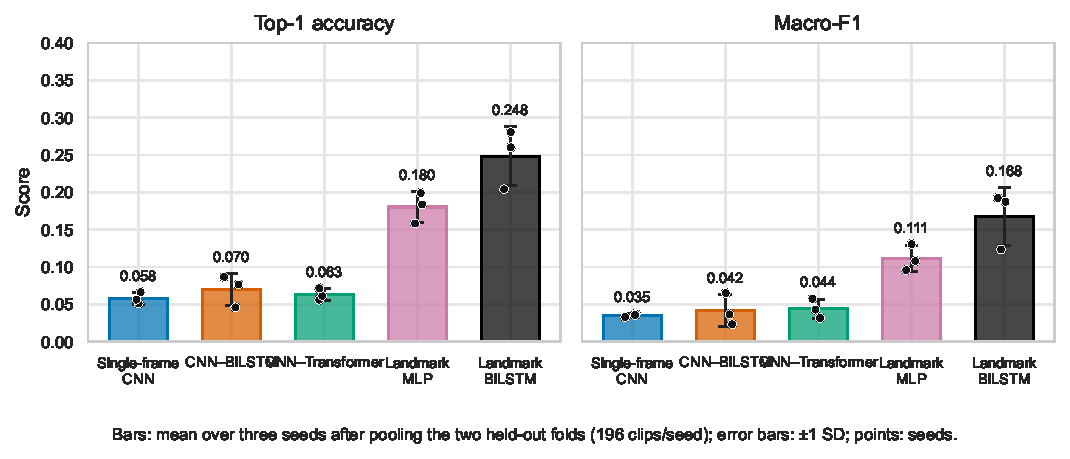
\includegraphics[width=0.98\linewidth]{figure_3_primary_performance.pdf}
\caption{Pooled cross-signer development accuracy and macro-F1. Bars are means over three seeds; error bars are one sample standard deviation; points are seeds.}
\label{fig:perf}
\end{figure}

\begin{figure}[t]
\centering
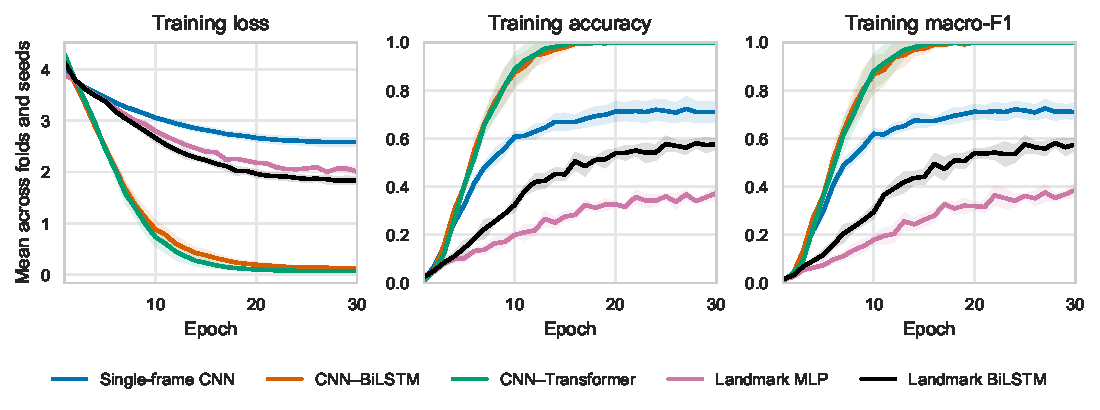
\includegraphics[width=0.98\linewidth]{figure_4_training_curves.pdf}
\caption{Training loss, accuracy, and macro-F1 (mean $\pm$ SD over folds and seeds). RGB temporal heads fit the training clips; landmark models do not reach training accuracy 1.}
\label{fig:train}
\end{figure}

\subsection{Landmark models}

The landmark MLP reaches $18.0\% \pm 2.1\%$ accuracy and $11.1\% \pm 1.8\%$ macro-F1. The landmark BiLSTM reaches $24.8\% \pm 4.0\%$ and $16.8\% \pm 3.8\%$. Relative to the single-frame CNN, the BiLSTM difference is $+19.0 \pm 3.7$ accuracy points and $+13.2 \pm 3.8$ macro-F1 points on the same 196 clips. Relative to the CNN--Transformer it is $+18.5 \pm 4.6$ and $+12.4 \pm 5.1$ points. The BiLSTM also leads the landmark MLP by $+6.8 \pm 1.9$ accuracy points.

Final-epoch training accuracy is $0.37 \pm 0.03$ for the MLP and $0.58 \pm 0.02$ for the landmark BiLSTM. Neither saturates the way the RGB temporal heads do.

Table~\ref{tab:folds} splits the two test people. Landmark BiLSTM is $25.9\% \pm 2.6\%$ on S1 and $23.8\% \pm 5.6\%$ on S2. The ordering versus RGB is the same in both folds.

\subsection{Lighting and sign type}

Table~\ref{tab:lighting} and Figure~\ref{fig:light} split the pre-specified bright and dark clips. Landmark BiLSTM is $27.6\% \pm 3.5\%$ on bright clips and $22.1\% \pm 4.6\%$ on dark clips. RGB models stay near $5$--$7\%$ in both conditions. The dark drop is a description of these files. We did not control illumination.

Table~\ref{tab:signtype} shows that most of the landmark gain occurs on vowels. RGB vowel accuracy is about $10\%$ for all three image models, so the temporal heads add little over the single-frame model on this subset. Landmark BiLSTM vowel accuracy is $66.0\% \pm 4.0\%$; consonant accuracy is $10.0\% \pm 3.9\%$. The MLP shows the same pattern at a lower level ($48.1\%$ vowels, $7.2\%$ consonants). Wrist and scale normalization alone leave most consonants misclassified.

\begin{figure}[t]
\centering
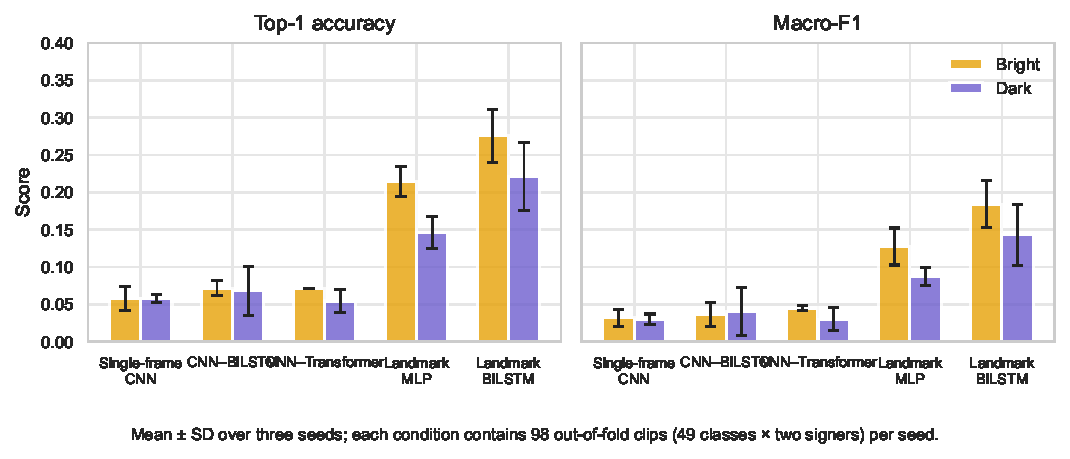
\includegraphics[width=0.98\linewidth]{figure_5_lighting_performance.pdf}
\caption{Bright versus dark accuracy and macro-F1. Each condition has 98 out-of-fold clips per seed.}
\label{fig:light}
\end{figure}

\begin{figure}[t]
\centering
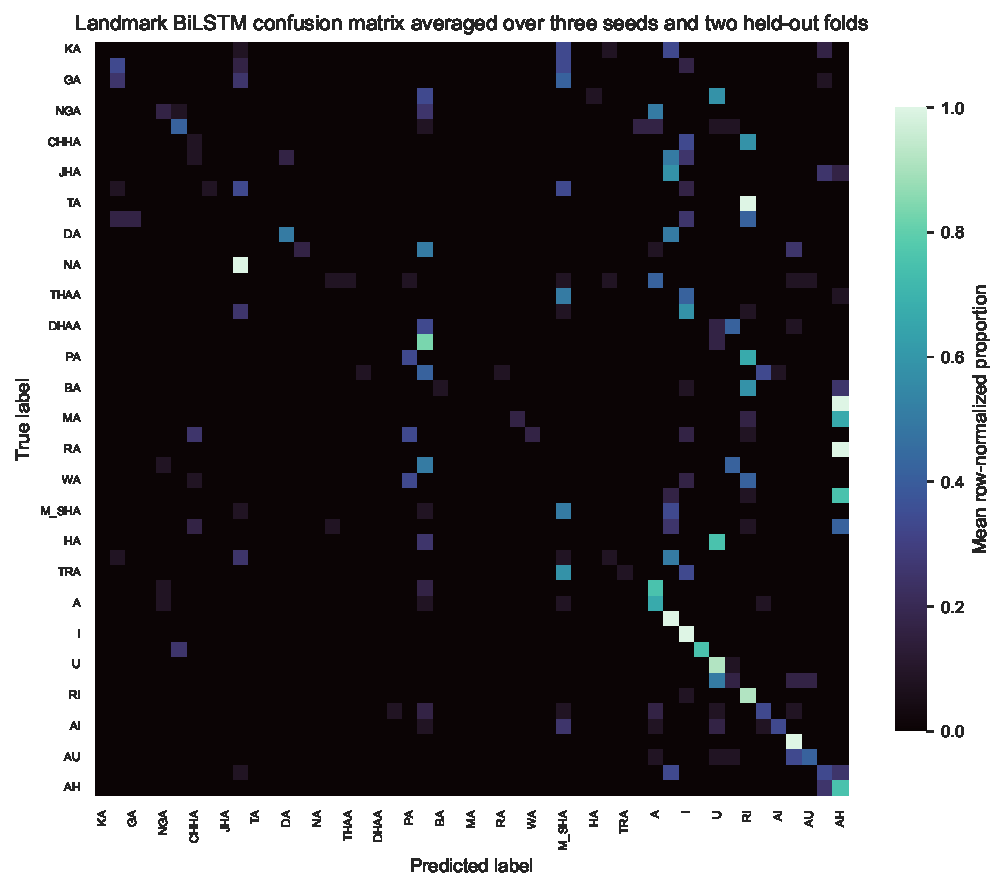
\includegraphics[width=0.98\linewidth]{figure_6_landmark_bilstm_confusion.pdf}
\caption{Landmark BiLSTM confusion, row-normalized and averaged over two folds and three seeds. Several consonants collapse onto a few vowel-like predictions.}
\label{fig:conf}
\end{figure}

\begin{figure}[t]
\centering
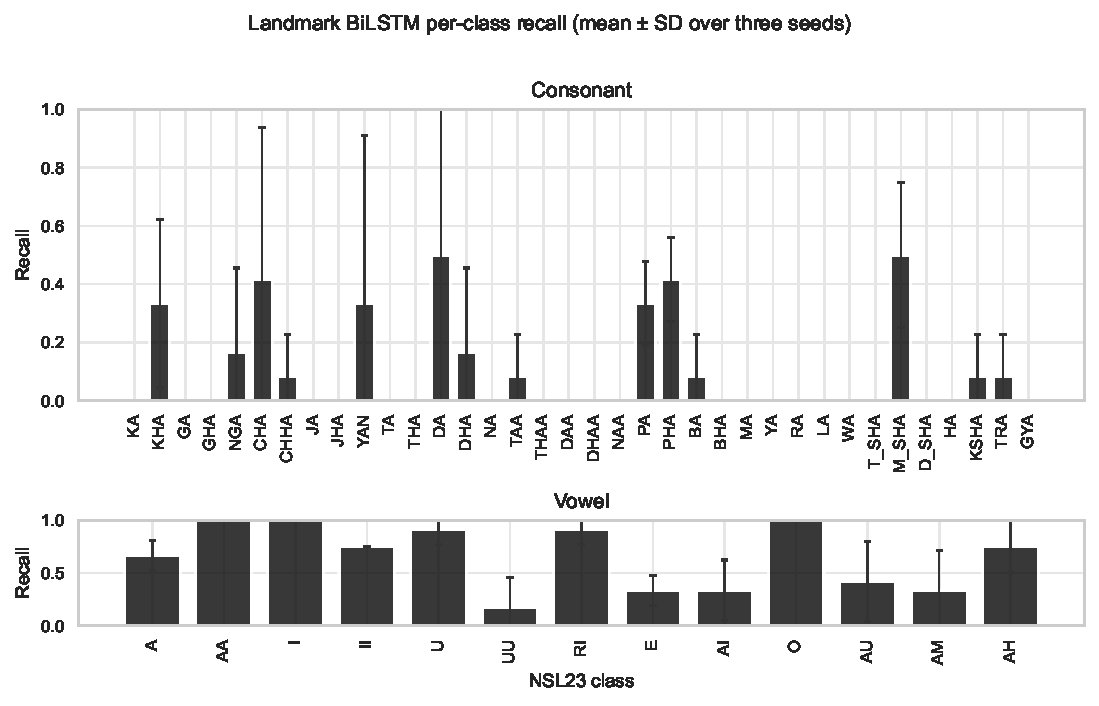
\includegraphics[width=0.98\linewidth]{figure_7_landmark_bilstm_per_class_recall.pdf}
\caption{Per-class recall of the landmark BiLSTM (mean $\pm$ SD over seeds). Vowels occupy the lower panel.}
\label{fig:recall}
\end{figure}

Figure~\ref{fig:conf} and Figure~\ref{fig:recall} show where consonants go. Across the 12 repeated evaluations of each class (two clips $\times$ two folds $\times$ three seeds), BHA, RA, and TA are never recognized. BHA and RA always map to AH; TA always maps to RI; NA always maps to YAN. Those confusions are stable on this protocol.

\subsection{Joint angles, prototypical classification, and crops}

Table~\ref{tab:improve} and Figure~\ref{fig:improve} report the follow-on matrix on the same 196 clips per seed. Concatenating the 20 angles under cross entropy raises the BiLSTM from $24.8\% \pm 4.0\%$ to $37.9\% \pm 2.4\%$. Consonant accuracy moves from $10.0\%$ to $28.7\% \pm 4.5\%$; vowels stay near $63.5\%$. The angle MLP does not beat the xyz BiLSTM.

The prototypical runs show a larger observed gain. An xyz prototypical BiLSTM reaches $55.8\% \pm 1.8\%$ accuracy and $53.4\% \pm 2.8\%$ macro-F1. Adding angles reaches $59.4\% \pm 3.3\%$ accuracy and $57.4\% \pm 3.6\%$ macro-F1. Consonants are $61.8\% \pm 5.7\%$; vowels are $52.6\% \pm 4.8\%$. Compared with the xyz softmax model, consonant accuracy increases while vowel accuracy falls. These runs also change the training schedule and prediction rule, so the difference cannot be attributed to the loss alone. Fold means are $63.3\% \pm 3.7\%$ on S1 and $55.4\% \pm 3.3\%$ on S2.

The cropped-hand CNN reaches $19.2\% \pm 1.3\%$, compared with $5.8\%$--$7.0\%$ for full-frame RGB. Equal-weight softmax fusion of the prototypical encoder and crop CNN reaches $59.7\% \pm 3.6\%$, only 0.3 percentage points above the prototypical encoder alone. Three seed scores provide insufficient evidence for a reliable fusion gain. Fusion of the angle BiLSTM and crop CNN is $41.5\% \pm 0.8\%$, above that BiLSTM's observed mean and below the prototypical result. Figure~\ref{fig:proto_conf} shows the prototypical confusion matrix.

% Auto-generated from the improvement matrix. Do not edit by hand.
\begin{table}[t]
\centering
\caption{Follow-on unseen-signer accuracy on the same S1/S2 folds (196 clips/seed; mean $\pm$ SD over three seeds). The xyz BiLSTM row is the frozen 30-run control.}
\label{tab:improve}
\small
\begin{tabular}{lcccc}
\toprule
Model & Acc. (\%) & Macro-F1 (\%) & Cons. (\%) & Vow. (\%) \\
\midrule
xyz BiLSTM (CE) & 24.8 $\pm$ 4.0 & 16.8 $\pm$ 3.8 & 10.0 $\pm$ 3.9 & 66.0 $\pm$ 4.0 \\
Hand-crop CNN & 19.2 $\pm$ 1.3 & 15.9 $\pm$ 0.7 & 15.5 $\pm$ 0.8 & 29.5 $\pm$ 2.9 \\
xyz+angle MLP (CE) & 22.4 $\pm$ 3.1 & 14.6 $\pm$ 2.9 & 13.7 $\pm$ 3.6 & 46.8 $\pm$ 2.9 \\
xyz+angle BiLSTM (CE) & 37.9 $\pm$ 2.4 & 30.1 $\pm$ 2.6 & 28.7 $\pm$ 4.5 & 63.5 $\pm$ 3.8 \\
xyz Proto-BiLSTM & 55.8 $\pm$ 1.8 & 50.6 $\pm$ 2.4 & 58.3 $\pm$ 2.5 & 48.7 $\pm$ 5.9 \\
xyz+angle Proto-BiLSTM & 59.4 $\pm$ 3.3 & 54.7 $\pm$ 4.2 & 61.8 $\pm$ 5.7 & 52.6 $\pm$ 4.8 \\
\bottomrule
\end{tabular}
\end{table}

\begin{table}[t]
\centering
\caption{Closed 1-shot enrollment: the other lighting of the held-out signer supplies one support clip per class (98 queries/fold). Mean $\pm$ SD over three seeds after pooling S1 and S2.}
\label{tab:enroll}
\small
\begin{tabular}{lcc}
\toprule
Encoder & Unseen signer (\%) & Closed 1-shot (\%) \\
\midrule
xyz BiLSTM (CE) & 24.8 $\pm$ 4.0 & 76.2 $\pm$ 4.2 \\
xyz+angle BiLSTM (CE) & 37.9 $\pm$ 2.4 & 78.2 $\pm$ 2.8 \\
xyz+angle Proto-BiLSTM & 59.4 $\pm$ 3.3 & 73.0 $\pm$ 1.5 \\
\bottomrule
\end{tabular}
\end{table}



\begin{figure}[t]
\centering
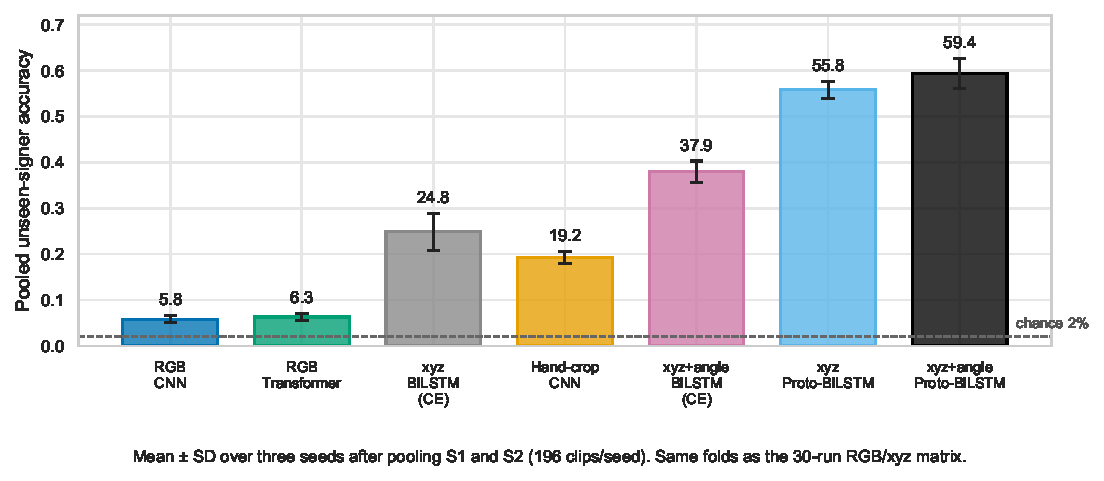
\includegraphics[width=0.98\linewidth]{figure_9_zero_shot_improvements.pdf}
\caption{Unseen-signer accuracy after pooling S1 and S2. The xyz BiLSTM is the frozen 30-run control; the remaining bars are the follow-on matrix.}
\label{fig:improve}
\end{figure}

\begin{figure}[t]
\centering
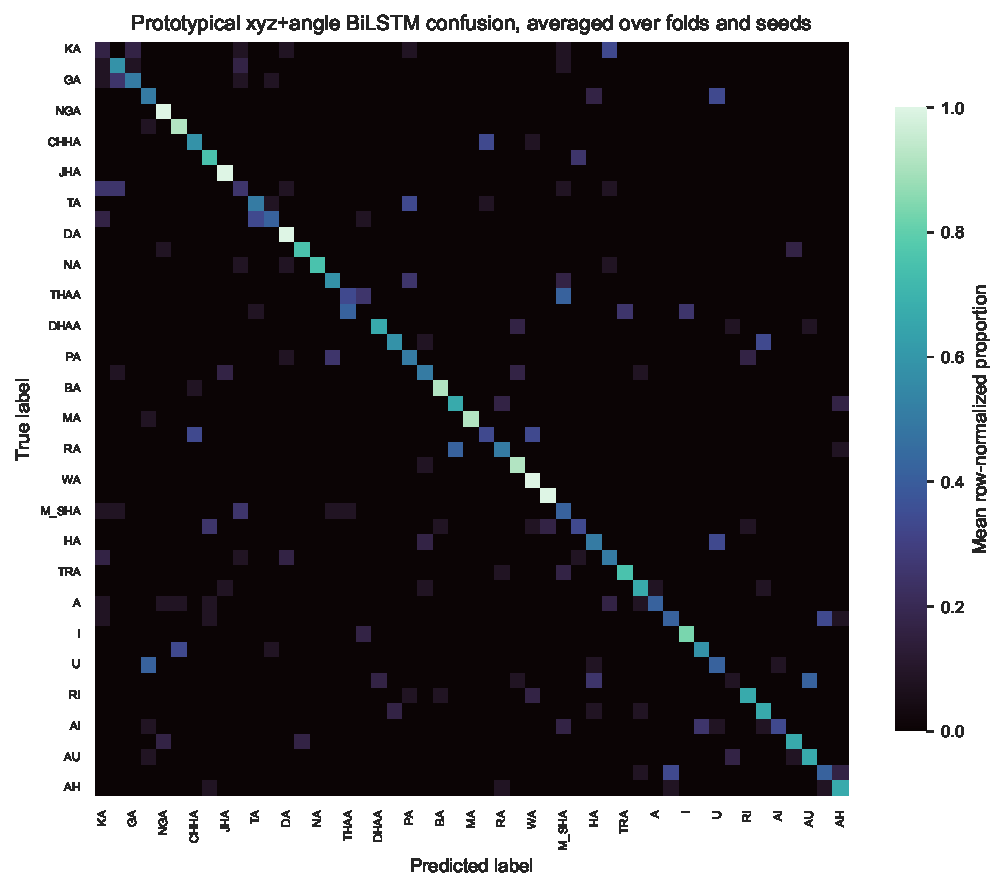
\includegraphics[width=0.98\linewidth]{figure_11_proto_bilstm_confusion.pdf}
\caption{Prototypical xyz+angle BiLSTM confusion, row-normalized and averaged over two folds and three seeds.}
\label{fig:proto_conf}
\end{figure}

\subsection{Closed 1-shot enrollment}

Table~\ref{tab:enroll} and Figure~\ref{fig:enroll} compare training-only classification with enrollment using the held-out signer's other lighting of every letter. Closed 1-shot accuracy is $76.2\% \pm 4.2\%$ for the xyz BiLSTM, $78.2\% \pm 2.8\%$ for the angle BiLSTM, and $73.0\% \pm 1.5\%$ for the prototypical encoder. The increases are larger for the softmax-trained encoders. Without enrollment, the prototypical encoder scores $59.4\%$ on this development sample; this does not establish the accuracy a future user would receive.

\subsection{Alternative evaluation protocols}

Table~\ref{tab:protocols} and Figure~\ref{fig:protocols} keep the encoder fixed and vary the candidate classes or scoring rule. This isolates how the evaluation task affects the reported percentage on these clips.

% Auto-generated alternative exams. Do not edit by hand.
\begin{table}[t]
\centering
\caption{The same xyz+angle prototypical encoder under alternative evaluation protocols. Scores describe S1/S2 development clips. Five-way evaluations use 500 draws per run; training means use all training clips of each selected class, while 1-shot uses one same-signer support clip per class.}
\label{tab:protocols}
\small
\begin{tabular}{lcc}
\toprule
Exam & Chance (\%) & Score (\%) \\
\midrule
49-way top-1, unseen signer (primary) & 2.0 & 59.4 $\pm$ 3.3 \\
49-way top-3, unseen signer & 6.1 & 85.5 $\pm$ 6.0 \\
49-way top-5, unseen signer & 10.2 & 91.3 $\pm$ 4.0 \\
36-way consonants, unseen signer & 2.8 & 65.7 $\pm$ 3.6 \\
5-way restriction, training-class means & 20.0 & 90.6 $\pm$ 2.5 \\
5-way 1-shot, same signer, other lighting & 20.0 & 93.3 $\pm$ 1.5 \\
49-way closed 1-shot, other lighting & 2.0 & 73.0 $\pm$ 1.5 \\
\bottomrule
\end{tabular}
\end{table}



Top-3 and top-5 ask whether the true class is among the nearest three or five prototypes ($85.5\% \pm 6.0\%$ and $91.3\% \pm 4.0\%$). Uniform-guessing rates are $6.1\%$ and $10.2\%$. Restricting both queries and candidate labels to the 36 consonants gives $65.7\% \pm 3.6\%$ (chance $2.8\%$). In 500 random five-class episodes per run, full training-class means give $90.6\% \pm 2.5\%$ on unseen-signer queries. This is a five-class restriction, not 1-shot evaluation: each mean uses every training clip of its class. A separate 5-way 1-shot setting uses one other-lighting support clip per class from the same signer and reaches $93.3\% \pm 1.5\%$ (chance $20\%$). Differences in support construction, modality, and dataset prevent direct comparison with Chamachot and Lertniphonphan's static-image few-shot scores~\cite{chamachot2026geometry}.

\begin{figure}[t]
\centering
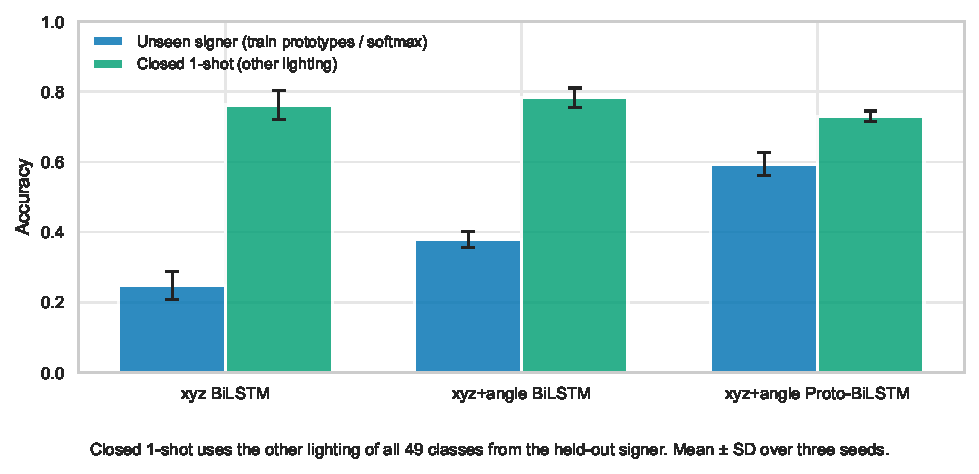
\includegraphics[width=0.98\linewidth]{figure_10_enrollment.pdf}
\caption{Unseen-signer classification versus closed 1-shot enrollment on the other lighting of the held-out signer.}
\label{fig:enroll}
\end{figure}

\begin{figure}[t]
\centering
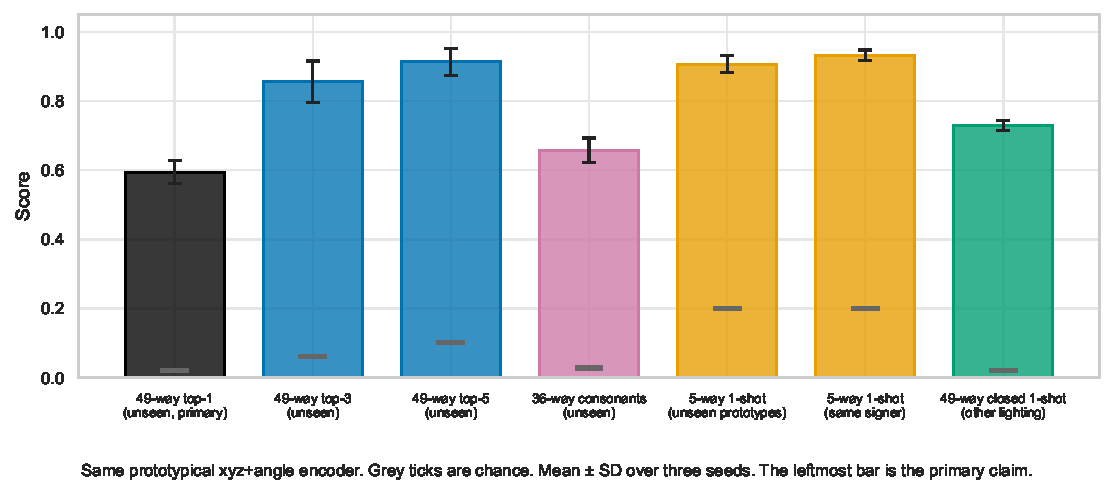
\includegraphics[width=0.98\linewidth]{figure_12_protocol_ladder.pdf}
\caption{Same prototypical encoder under different evaluation tasks. Grey marks are uniform-guessing rates. The leftmost bar is the 49-way unseen-signer top-1 development result.}
\label{fig:protocols}
\end{figure}

\subsection{Runtime and webcam}

Table~\ref{tab:runtime} separates network time from pipeline time. On MPS, RGB model-only medians are $4.0$~ms (single-frame) and about $50$~ms (temporal heads). End-to-end RGB clip processing is about $0.94$--$0.97$~s because decoding dominates. A camera frame rate would have to count frames from a live stream, which this column does not.

On CPU, the landmark BiLSTM forward pass is $0.3$~ms per 16-frame clip ($0.5$~ms at the 95th percentile). MediaPipe on those 16 cached frames plus the classifier takes a median $346$~ms per clip. The webcam loop is cheaper per frame because Hands runs in video mode on one frame at a time and the LSTM sees a rolling window.

On original NSL23 videos, with the prototypical xyz+angle encoder trained without the signer in the file, the loop processed 90 frames of S1's bright isolated \texttt{A} in $2.27$~s ($39.6$~FPS). The argmax after EMA smoothing was \texttt{A}. The earlier xyz softmax loop on the same clip was $39.7$~FPS; nearest-prototype classification leaves the MediaPipe-dominated budget almost unchanged. Three earlier xyz-softmax streams (S1 bright, S1 dark, S2 bright \texttt{A}) ran at $33$--$42$~FPS. That is a speed check on one vowel.

\section{Discussion}

With a frozen ImageNet MobileNetV2 encoder and 16 letterboxed frames, the BiLSTM and Transformer heads achieve little improvement over the single-frame baseline. Their training accuracy reaches $1.00$ while evaluation stays near $6\%$. The result is consistent with overfitting and limited feature transfer. It does not show that temporal models are generally ineffective for sign recognition, or establish whether hand resolution, background cues, or another feature limitation caused the errors.

The landmark BiLSTM improves the observed mean to $24.8\%$. Its 64-dimensional input removes direct RGB background information, although detector outputs can still vary with recording conditions. Most correct predictions are vowels ($66\%$ versus $10\%$ on consonants). BHA, RA, and TA are never predicted correctly across their twelve repeated evaluations, which limits the model's usefulness for alphabet practice.

The xyz+angle prototypical encoder reaches $61.8\%$ on consonants and $59.4\%$ overall. Roughly two in five evaluation clips remain incorrect. Closed 1-shot scores of $76$--$78\%$ for the softmax-trained encoders require a labelled recording of every class from the same signer and session. Each direction uses one lighting for support and the other for queries. These results use signer-specific information unavailable in the training-only protocol and should be reported separately.

Cropping raises the frozen CNN's observed accuracy to $19.2\%$, suggesting that hand localization matters in this setup. The remaining errors warrant further comparisons with fine-tuned or hand-specific encoders; they do not isolate the cause of the RGB model's poor transfer.

Other NSL and few-shot studies use different vocabularies, source collections, and support sets~\cite{heuju2022word,shrestha2024mediapipe,chamachot2026geometry}. Table~\ref{tab:protocols} illustrates the effect of narrowing the candidate classes within this study, rather than providing a leaderboard across those papers. The $59.4\%$ result remains an exploratory estimate on the fixed S1/S2 development clips.

\section{Limitations}

S1 and S2 are the entire complete-alphabet cross-signer development set. They were held out within each training run, but they also informed the later angle, crop, prototypical, and fusion comparisons. Bootstrap intervals on 196 clips describe those clips; they neither restore an untouched test nor describe a population of signers. The five prepared-consonant people never sit in the complete-alphabet evaluation seat. Outdoor and real-world files in the Zenodo dump were left out of the primary sample because they fail the original-isolated-labelled audit. The clips themselves are isolated one-handed letters; sentence-level fingerspelling and body-relative signs are absent.

MediaPipe returned landmarks on $97.8\%$ of the $6{,}000$ cached frames, with no empty clips. This measures output availability, not landmark accuracy. Detector performance across new cameras, lighting, and skin tones was not measured. The detector and settings remained fixed throughout the study.

The RGB encoder remained frozen as a controlled baseline. Fine-tuning MobileNetV2 and pretraining on separate letter images were not tested. The results therefore do not establish the best achievable RGB accuracy. Hyperparameters were fixed before the RGB matrix and may be suboptimal. Prototypical training also used 40 epochs rather than 30 and a different sampling scheme; its support/query overlap during training limits interpretation of the nominal shot counts.

Enrollment here is the other lighting of the same session. There is no second-day recording and no live enrollment UI. Two clips per class per signer also means 5-shot enrollment of the test person has no honest support set.

The FPS numbers come from replaying NSL23 \texttt{.MOV} files on an Apple~M4 with MediaPipe~0.10.14 on CPU. A live user study would be a different paper. Interactive speed and recognition quality are separate measurements.

\section{Conclusion}

The xyz+angle prototypical BiLSTM achieves $59.4\% \pm 3.3\%$ accuracy on 196 pooled S1/S2 evaluation clips drawn from the 375 audited original isolated NSL23 clips. Consonant accuracy is $61.8\%$. The frozen RGB baselines reach $5.8\%$--$7.0\%$, and the xyz landmark BiLSTM reaches $24.8\%$. Recorded-video streaming checks on an Apple~M4 CPU process $33$--$42$ frames per second, with recognition accuracy assessed separately on isolated clips. Reuse of the two complete-alphabet signers for follow-on development limits the result to this exploratory sample. The next study needs a prospectively locked signer cohort; evaluation in Nepal would also require local data. Code, folds, and predictions are available in the \href{https://github.com/twasanon/nsl23-low-resource-alphabet}{project repository}.

\section*{Data availability}

NSL23 videos are distributed by Sunuwar, Borah, and Kharga under CC~BY~4.0~\cite{sunuwar2023zenodo,sunuwar2024nsl23}. This repository does not republish the archives. Code, portable fold manifests, landmark caches, checkpoints, tabulated results, the immutable Version~1 snapshot, its historical-tree verifier, and the Version~2 annotation protocol are in the \href{https://github.com/twasanon/nsl23-low-resource-alphabet}{project repository}.

\section*{Acknowledgements}

The recordings were collected and released by the NSL23 authors. This paper is a secondary analysis of those files.

\begingroup
\small
\singlespacing
\bibliographystyle{plainnat}
\bibliography{references}
\endgroup

\end{document}
